% Template for Cogsci submission with R Markdown

% Stuff changed from original Markdown PLOS Template
\documentclass[10pt, letterpaper]{article}

\usepackage{cogsci}
\usepackage{pslatex}
\usepackage{float}
\usepackage{caption}

% amsmath package, useful for mathematical formulas
\usepackage{amsmath}

% amssymb package, useful for mathematical symbols
\usepackage{amssymb}

% hyperref package, useful for hyperlinks
\usepackage{hyperref}

% graphicx package, useful for including eps and pdf graphics
% include graphics with the command \includegraphics
\usepackage{graphicx}

% Sweave(-like)
\usepackage{fancyvrb}
\DefineVerbatimEnvironment{Sinput}{Verbatim}{fontshape=sl}
\DefineVerbatimEnvironment{Soutput}{Verbatim}{}
\DefineVerbatimEnvironment{Scode}{Verbatim}{fontshape=sl}
\newenvironment{Schunk}{}{}
\DefineVerbatimEnvironment{Code}{Verbatim}{}
\DefineVerbatimEnvironment{CodeInput}{Verbatim}{fontshape=sl}
\DefineVerbatimEnvironment{CodeOutput}{Verbatim}{}
\newenvironment{CodeChunk}{}{}

% cite package, to clean up citations in the main text. Do not remove.
\usepackage{cite}

\usepackage{color}

% Use doublespacing - comment out for single spacing
%\usepackage{setspace}
%\doublespacing


% % Text layout
% \topmargin 0.0cm
% \oddsidemargin 0.5cm
% \evensidemargin 0.5cm
% \textwidth 16cm
% \textheight 21cm

\title{Communicative pressure can lead to input that supports language learning}


\author{{\large \bf Benjamin C. Morris} \\ \texttt{benmorris@uchicago.edu} \\ Department of Psychology \\ University of Chicago \And {\large \bf Daniel Yurovsky} \\ \texttt{yurovsky@uchicago.edu} \\ Department of Psychology \\ University of Chicago}

\begin{document}

\maketitle

\begin{abstract}
Infants prefer to listen to and learn better from child-directed speech.
This speech might support learning in part due to communicative
pressure: parents must use language that their children understand. We
designed a Mechanical Turk study to experimentally validate this idea,
putting Turkers in the role of parents talking with children who knew a
novel language less well. Participants could communicate in 3 ways:
pointing---expensive but unambiguous, labelling---cheap but
knowledge-dependent, or both. They won points only for communicating
successfully; using pointing and labelling together was costly, but
could teach, allowing cheaper communication on later trials.
Participants were modulated their communicate behavior in response to
their own and their partner's knowledge and teaaching emerged when the
speaker had substanially more knowledge of the lexicon. While language
is more than reference games, this work validates the hypothesis that
communicative pressure alone can lead to supportive language input.

\textbf{Keywords:}
Language; Child-Directed Speech; POMDP.
\end{abstract}

\section{Introduction}\label{introduction}

One of the most striking aspects of children's language learning is just
how quickly they master the complex system of their natural langauge
(Bloom, 2000). In just a few short years, children go from complete
ignorance to conversational fluency that is the envy of second-language
learners attempting the same feat later in life (Newport, 1990). What
accounts for this remarkable transition?

One possiblility is that children's caregivers deserve most of the
credit; that the language parents produce to their children is optimized
for teaching. Although there is some evidence that aspects of
child-directed speech support learning, other aspects--even in the same
subproblem, e.g.~phoneme discrimination--appear to make learning more
difficul (Eaves Jr, Feldman, Griffiths, \& Shafto, 2016; McMurray,
Kovack-Lesh, Goodwin, \& McEchron, 2013). In general, parents rarely
explicltly correct their children, and children are resistant to the
rare explicit language correction they do get (Newport, Gleitman, \&
Gleitman, 1977). Thus while parents may occasionally offer a supervisory
signal, the bulk of the evidence suggests that parental supervision is
unlikely to explain rapid early language acqusition.

Alternatively, even the youngest infants may already come to language
acquisition with a precocious ability to learn the latent structure of
language from the statistical properties of the language in their
ambient environment (Saffran \& 2003, 2003; L. B. Smith \& Yu, 2008).
While a number of experiments clearly demonstrate the early availability
of such mechanisms, there is reason to be suspicious about just how
precocious they are early in development. For example, infants' ability
to track the co-occurrence information connecting words to their
referents appears to be highly constrained by both their developing
memory and attention systems (L. B. Smith \& Yu, 2013; Vlach \& Johnson,
2013). Further, computational models of these processes show that the
rate of acquisition is highly sensitive to variation in environmental
statistics (Blythe, Smith, \& Smith, 2010; Vogt, 2012). Thus precocious
unsupervised statistical learning also appears to fall short of an
explanation for rapid early language learning.

In this paper we explore the consequences of a a third possibility: The
language that children hear is neither designed for pedagogy, nor is it
random: it is designed for communication (Brown, 1977). We take as the
caregiver's goal the desire to communicate with the child, not about
language itself, but instead about the world in front of them. To
succeed, the caregiver must produce the kinds of commincative signals
that the child can understand, and thus might tune the complexity of
their speech not for the sake of learning itself, but as a byproduct of
in-the-moment pressure to communicate successfully (Yurovsky, 2017).

We explore the emergence of tuning in a simple model system: an iterated
reference game in which two players earn points for communicating
successfully with each-other. On each round of the game, participants
can point--a signal which is costly to produce but always
communicatively effective, or can use language--a cheaper signal which
is cheap to produce but successful only if both players share a common
lexicon. Crucially, participants can point and speak together--paying
the cost of both, but effectively establishing a shared label for this
referent that they can exploit on later trials of the game.

In a series of experiments on Mechanical Turk, we show that people tune
their communicative to choices to varying cost and reward structures,
and also critically to their partner's linguistic knowledge--teaching
when partners are unlikely to know language and many more rounds remain.
We then show that human behavior can be explained by a rational planning
model that seeks to optimize its expected utility over the course of the
game. Together, this shows that pedagogically-supportive input can arise
from purely selfish motives to maximize the cost of communicating
successfully while minimizing the cost of communcation. We take these
results as a proof of concept that both the features of child-directed
speech that support learning as well as those that inhibit it may arise
from a single unifying goal: The desire to communicative efficiently.

\section{Model: Communication as
Planning}\label{model-communication-as-planning}

We implemented a two-agent model of speaker and listener behavior in
this game based on partially observable Markov decision processes. The
speaker is given a target referent each trial and must signal to the
listener which object to select. Speakers send messages to the listener
by speaking, a low cost cue that relies on the listener's knowledge, or
by pointing, a higher cost cue that is unambiguous.

The speaker estimates the listener's knowledge. First, the speaker uses
Markov chain Monte Carlo to infer their own learning rate based on how
well they were able to learn a novel lexicon after N exposures. Then,
given the listner's degree of exposure, the speaker can use their own
learning rate to infer the probability that the listener would know any
given object-label mapping. Across trials, the speaker gains further
information about the listener through their selections, allowing them
to update their beliefs about the listener's knoweldge state.

The model specifies the relative costs for each communicative modality.
On each trial, the speaker estimates the expected utility of each
modality by accounting for these costs, their own knowledge of the
object's label, and the probability that the listner knows the object's
label. The speaker then uses Luce's choice axiom to select a
communicative modality based on the expected utilities.

When estimating expected utility, the model sums the expected utility of
a given trial and any remaining trials for that particular object. This
allows the speaker to engage in planning by accounting for the way a
given message may induce knowledge changes and thus affect subsequent
expected utilities. Utilites were scaled using an exponential discounter
as a function of delay (Do we want to cite a precedent for this?) to
give greater weight to immediate rewards than subsequent rewards.

Crucially, speakers can also combine both communication cues, paying the
upfront cost of both, to produce a message that is both unambiguous and
informative. In this way, speakers are able to teach their partners
object-label mappings. A speaker that plans may thus infer that teaching
the listener, especially if there is an asymmetry in their knowledge
states, may have a high expected utility after accounting for remaining
trials where the speaker could use a less costly cue (i.e.~speech).
After producing both cues, the speaker also updates their own beliefs
about the partner's knowledge state to reflect this exposure.

Over the course of three experiments, {[}TOTAL N{]} participants were
recruited via Amazon Mechanical Turk, an online platform that allows
workers to complete surveys and short tasks for payment. Turkers played
partnered, iterated reference games. In these studies, all particpants
were placed in the role of speaker and listener responses were
programmed.

\section{Experiment 1a}\label{experiment-1a}

Our model's speaker chooses a communicative modality by optimizing the
expected utilities of the possible modalities. By manipulating the
utility of each strategy, we can evaluate our models predictions about
the extent to which speakers sensibly adapt to these imposed utilites.
In this experiment, we explicitly implemented strategy utility by
assigning point values to each strategy.

\subsection{Participants, Materials,
Methods}\label{participants-materials-methods}

{[}n{]} particpants were recruited though Amazon Mechanical Turk and
received a small payment for their participation.

Participants were told they would be introduced to novel object-label
pairs and then asked to play a communication game with a partner wherein
they would have to refer to a particular target object. Particpants were
exposed to nine novel objects, each with a randomly assigned pseudoword
label. We manipulated the degree of exposure within subjects, such that,
during training, particpants saw three of the nine object-label mappings
four times, two times, or one time, resulting in a total of 27 training
trials. Participants were then given a simple recall task to establish
their baseline knowledge of the novel lexicon.

After being introduced to the rules of the game, participants were told
they would be asked to communicate about each object three times. During
gameplay, speakers saw the target object in addition to an array of all
nine objects. Speakers had the option of either directly selecting the
target object from the array (gesture)- a higher cost cue but without
ambiguity- or typing a label for the object (speech)- a lower cost cue
but contingent on the listener's knowledge. After sending the message,
speakers are shown which object the listener selected.

If the speaker clicked on on object (gesture message), the listener was
coded to simply make the same selection. If the speaker typed an object
label, the listener evaluated the Levenshtein distance (LD) between the
typed label and each of the nine possible labels and selected the
candidate with the smalles edit distance. If none of the nine object
labels had an LD less than or equal to two, the listener always selected
an incorrect object.

Speakers could win up to 100 points per trial if the listener correctly
selected the target referent based on their message. If the listener
failed to identify the target object, the speaker received no points. We
manipulated the relative utilities of each of the strategies
between-subjects. In the `Talk is Cheap' condition, speakers recieved 30
points for gesturing and 100 points for labeling, while in the `Talk is
Less Cheap' condition speakers recieved 50 points for gesturing and 80
points for labeling.

\subsection{Results}\label{results}

As expected, particpants were sensitve to both the exposure rate and the
relative utilities of the communication strategies. Speakers produced
significantly more labels for object-label mappings that were shown more
frequently during training than for the mappings that were less frequent
(\ldots{}). The reverse was true for gesture (\ldots{}). The more
exposures to a given object-label pair during training, the more likely
participants were to recall that label at pretest (\ldots{}). The effect
of exposure rate on modality choice held even after controlling for
pretest knowledge, indicating the effect was more than the result of
being constrained by knowledge of the label (\ldots{}). \ldots{}{[}I'm
not sure which statistics to include here, since most of what i'd been
looking at are these logitistic regression models with all our
predictors.Should I subset to just one partners exposure, and then do
the logistic regression with exposure rate, utility condition,
appearance, and the random effect? Does that make sense?{]}\ldots{}

Participants also modulated their communicative behavior on the basis of
the utility manipulation. Speakers in the Talk is Cheap condition
produced significantly more labels than particpants in the Talk is Less
Cheap condition (\ldots{}). Again, this effect was reversed for gesture
(\ldots{}). Thus, participants are senstive to our manipulations-
altering their choices about how to communicate with their partner on
the basis of their own knowledge, the degree of training, and the
imposed utilities.

\begin{CodeChunk}
\captionsetup{width=0.8\columnwidth}\begin{figure}[H]

{\centering 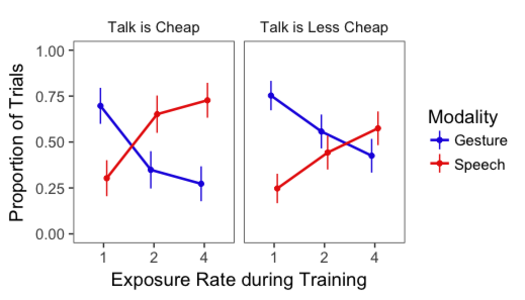
\includegraphics{figs/image1-1} 

}

\caption[Plot of modality choice as a function of exposure, split by utility condition]{Plot of modality choice as a function of exposure, split by utility condition.}\label{fig:image1}
\end{figure}
\end{CodeChunk}

\section{Experiment 1b}\label{experiment-1b}

As a replication and extension of Experiment 1a, we sought to embed the
relative utilites of the communicative strageies in the game more
implicitly. In experiment 1b, we used the same procedure described
above; however, a timer controlled the number of points that were earned
on each trial of gameplay. Rather than impose an explicit point system
as in Experiment 1a, we set the relative utilities of communication
strategies by manipulating the speed with which particpants could
respond.

\subsection{Participants, Materials,
Methods}\label{participants-materials-methods-1}

{[}n{]} particpants were recruited though Amazon Mechanical Turk and
received a small payment for their participation.

Experiment 1b utilitzed the same training and pretest procedures, but
gameplay differed in a number of ways. During the game, the nine novel
objects were arranged in a circle around a cartoon pointer (see Figure
2). To manipulate the relative speeds of gesturing and labeling, we
required speakers to move the small pointer with the arrow keys on their
keyboards in order to select an object with gesture. With this method we
could directly manipulate the speed of the pointer while holding the
arrow keys to effectively set maximum possible utility of using gesture.

\begin{CodeChunk}
\captionsetup{width=0.8\columnwidth}\begin{figure}[H]

{\centering 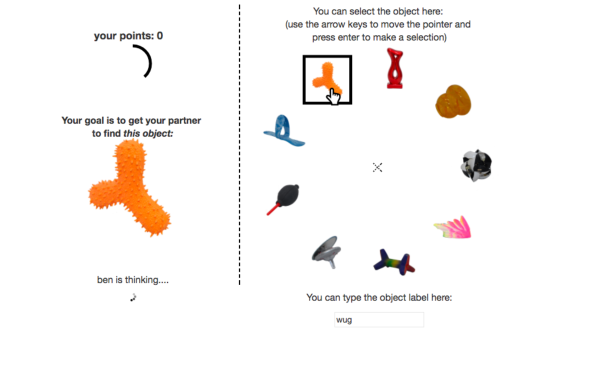
\includegraphics{figs/image-1} 

}

\caption[Screenshot of speaker view during gameplay]{Screenshot of speaker view during gameplay.}\label{fig:image}
\end{figure}
\end{CodeChunk}

If the listner correctly identified the target object, speakers recieved
points determined by the amount of time remaining on the timer. For
successful communications, speakers always recieved a minimum of 10
points, regardless of the time elapsed. Based on pilot response times,
the timer was set to 6.5 seconds and points were scaled to match
Experiment 1a. Participants were randomly assigned into one of three
conditions, where the pointer was set to either a fast, slow, or slowest
setting.

This framework allowed us to implement the point system as an implicit
extension of gameplay and resulted in each partipcant having unique
gesture-speech utilities, based on their speed of responses across the
two methods.

\subsection{Results}\label{results-1}

As expected, the same patterns emerge as experiment 1a. Speakers again
labeled signifcantly more (TBD) and gestured significantly less (TBD) on
high exposure targets, relative to low exposure targets. Particpants
were signficantly more likely to recall the high exposure labels than
the low exposure labels at pretest (TBD), and this effect did not
account the effect of exposure rate on modality choice (TBD).

Critically, there was a main effect of our utility manipulation, such
that speakers in the fast pointer condition produced signficantly more
gestures than particpants in the slowest pointer condition (TBD). The
pattern is reveresed for labeling (TBD). In the absence of an explicit
framework for assigning utilities based on method, speakers continue to
adapt their communicative choices taking into account the expected
utility of possible strategies.

\section{Experiment 2a}\label{experiment-2a}

{[}I don't know how to divvy up these ns{]}

{[}n{]} particpants were recruited though Amazon Mechanical Turk and
received a small payment for their participation.

Thus far, we have focused on relatively straightforward scenarios to
demonstrate that a pressure to communicate successfully in the moment
can lead speakers to trade-off between gesture and speech sensibly.
However, critical to these repeated interactions is the ability to learn
about an interlocuter and potentially influence their learning. In
Experiment 2a, particpants could send a third type of message by
utilizing both gesture and speech within a single trial to effectively
teach the listener an object-label mapping.

\subsection{Participants, Materials,
Methods}\label{participants-materials-methods-2}

In order to produce teaching beahvior, speakers had to pay the cost of
producing both cues, yeilding 30 points in either conditon of our
explicit points framework. Our communicative game was designed to reward
in-the-moment communication, and teaching required the speaker paying a
cost upfront. However, rational communicators may understand that if one
is accounting for future trials, paying the cost upfront to teach the
listener allows a speaker to use a less costly message strategy on
subsequent trials.

Incorporating teaching means that our speaker must now reason about
their interlocuter's knoweldge state more explicitly, in order to make
rational decisions about what to teach and when. To address this added
dimension, we also manipulated participants expectations about their
partner's knowledge. Prior to beginning the game, participants were told
that there partner had no experience with the lexicon, had half the
experience of the speaker, or had twice the experience of the speaker.

Listener starting knowledge state was also initialized accordingly.
Listners with no exposure were given no knowledge of the lexicon to
start. Listners with half the exposure of the speaker began with
knowledge of three object-label pairs (2 high frequency, 1 mid
frequency), based the typical retention rates found previously. Lastly,
the listener with twice as much exposure as the speaker began with
perfect knowledge of the lexicon. Through gesture-speech co-occurance,
the speaker could effectively teach the listener a novel mapping.
Listners could learn a novel mapping from one teaching event in this
game and integrate it into their set of candidate words when evaluating
the LD of subsequent labels.

{[}I'm not sure how to describe the methods here{]}. {[}Experiment 2a
directly mirrored Experiment 1a, except that partipcants were introduced
to an additional strategy, i.e.~teaching, during the introduction to the
game (feels a little wonky).{]}

\subsection{Results}\label{results-2}

As predicted, mixed effects logistic regression predicting whether or
not teaching occured on a given trial revealed that teaching rates
across conditions depend on all of the same factors that predict speech
and gesture. There was a signficant effect of intial exposure to the
mapping on the rates of teaching, such that more exposures to a word
predicted higher rates of teaching behavior (B = 0.09, p = 0.045). There
was also a signficant effect of the utility manipluation such that being
in the Talk is Less Cheap condition predicted lower rates of teaching
than being in the Talk is Cheap condtion (B = -0.98, p \textless{}
0.01), a rational response considering the eventual benefit for teaching
a novel word is less strong in this former condition.

We also included whether this was an objects first, second, or third
appearance as a predictor in our model. The expected utility of teaching
on a given trial should decrease as there are fewer subsequent trials
for that object, thus we predicted that teaching rates would drop
dramatically. Indeed, this is consistent with the results from our
model; compared with the first appearance of an object, speakers were
significantly less likely to teach on the second appearance (B = -1.11,
p \textless{} 0.001) or the third appearance (B = -2.01, p \textless{}
0.001).

Interestingly, as we expected, there was a signficant effect of our
manipulation of listener knowledge. Compared with listner's with no
experience with the lexicon, speakers were signifcantly less likely to
teach when they were told the listner had half as much exposure (B =
-1.19, p \textless{} 0.01) or twice as much exposure as they themselves
did (B = -4.64, p \textless{} 0.001).

\begin{CodeChunk}
\captionsetup{width=0.8\columnwidth}\begin{figure}[H]

{\centering 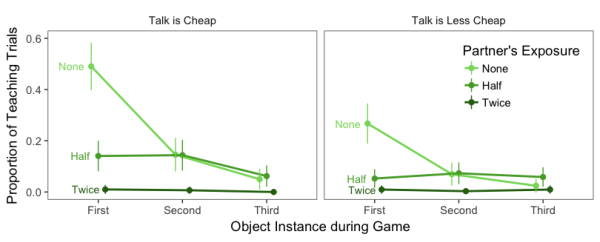
\includegraphics{figs/image3-1} 

}

\caption[Proportion of teaching behavior as a function of whether it was the first, second, or third appearance of a given target, split by partner's level of exposure]{Proportion of teaching behavior as a function of whether it was the first, second, or third appearance of a given target, split by partner's level of exposure.}\label{fig:image3}
\end{figure}
\end{CodeChunk}

\section{Experiment 2b}\label{experiment-2b}

We investigated the emergence of teaching in both a paradigm with an
explicit points system (Experiment 2a) and an implicit points system
(Experiment 2b).

\subsection{Participants, Materials,
Methods}\label{participants-materials-methods-3}

\subsection{Results}\label{results-3}

\section{Experiment 3}\label{experiment-3}

Planning is critical to our model. A pressure to communicate
successfully in-the-moment can lead to pedagogical-like input without
pedagogical goals, merely by wishing to communicate more efficiently in
the future. As a final check to ensure that accounting for the future is
indeed crucial to the emergence of pedagoical behaviors in our
framework, we ran a version of our partnered game where speakers are
told they will only send emssages about each object 1 time.

As expected, teaching behavior dropped off completely\ldots{} (TBD).

\section{Model Comparison}\label{model-comparison}

{[}Is this where the actual model fit stuff should live?{]}

\begin{CodeChunk}
\captionsetup{width=0.8\columnwidth}\begin{figure}[H]

{\centering 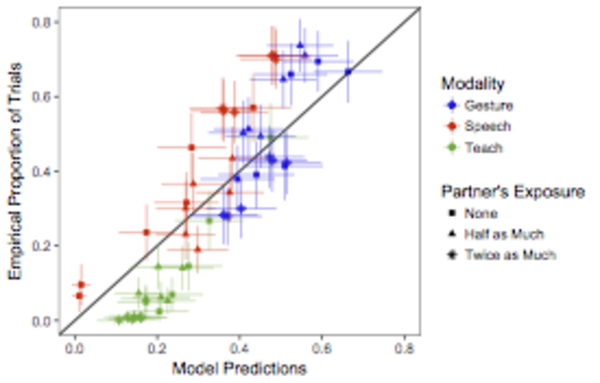
\includegraphics{figs/image4-1} 

}

\caption[Plot of the fit between model predictions and empirical data]{Plot of the fit between model predictions and empirical data.}\label{fig:image4}
\end{figure}
\end{CodeChunk}

\section{Discussion}\label{discussion}

\section{Acknowledgements}\label{acknowledgements}

Place acknowledgments (including funding information) in a section at
the end of the paper.

\section{References}\label{references}

\setlength{\parindent}{-0.1in} \setlength{\leftskip}{0.125in} \noindent

\hypertarget{refs}{}
\hypertarget{ref-bloom2000}{}
Bloom, P. (2000). \emph{How children learn the meanings of words}. MIT
press: Cambridge, MA.

\hypertarget{ref-blythe2010}{}
Blythe, R. A., Smith, K., \& Smith, A. D. M. (2010). Learning times for
large lexicons through cross-situational learning. \emph{Cognitive
Science}, \emph{34}, 620--642.

\hypertarget{ref-brown1977}{}
Brown, R. (1977). Introduction. In C. E. Snow \& C. A. Ferguson (Eds.),
\emph{Talking to children: Language input and interaction}. Cambridge,
MA.: MIT Press.

\hypertarget{ref-eaves-jr2016}{}
Eaves Jr, B. S., Feldman, N. H., Griffiths, T. L., \& Shafto, P. (2016).
Infant-directed speech is consistent with teaching. \emph{Psychological
Review}, \emph{123}(6), 758.

\hypertarget{ref-mcmurray2013}{}
McMurray, B., Kovack-Lesh, K. A., Goodwin, D., \& McEchron, W. (2013).
Infant directed speech and the development of speech perception:
Enhancing development or an unintended consequence? \emph{Cognition},
\emph{129}(2), 362--378.

\hypertarget{ref-newport1990}{}
Newport, E. L. (1990). Maturational Constraints on Language Learning.
\emph{Cognitive Science}, \emph{14}(1), 11--28.

\hypertarget{ref-newport1977}{}
Newport, E. L., Gleitman, H., \& Gleitman, L. R. (1977). Mother, I'd
rather do it myself: Some effects and non-effects of maternal speech
style. In C. A. Ferguson (Ed.), \emph{Talking to children language input
and interaction} (pp. 109--149). Cambridge University Press.

\hypertarget{ref-saffran2003}{}
Saffran, J. R., \& 2003. (2003). Statistical language learning:
Mechanisms and constraints. \emph{Current Directions in Psychological
Science}, \emph{12}(4), 110--114.

\hypertarget{ref-smith2008}{}
Smith, L. B., \& Yu, C. (2008). Infants rapidly learn word-referent
mappings via cross-situational statistics. \emph{Cognition}, \emph{106},
1558--1568.

\hypertarget{ref-smith2013}{}
Smith, L. B., \& Yu, C. (2013). Visual attention is not enough:
Individual differences in statistical word-referent learning in infants.
\emph{Language Learning and \ldots{}}, \emph{9}, 25--49.

\hypertarget{ref-vlach2013}{}
Vlach, H. A., \& Johnson, S. P. (2013). Memory constraints on infants’
cross-situational statistical learning. \emph{Cognition}, \emph{127}(3),
375--382.

\hypertarget{ref-vogt2012}{}
Vogt, P. (2012). Exploring the robustness of cross-situational learning
under zipfian distributions. \emph{Cognitive Science}, \emph{36}(4),
726--739.

\hypertarget{ref-yurovsky2017}{}
Yurovsky, D. (2017). A communicative approach to early word learning.
\emph{New Ideas in Psychology}, 1--7.

\end{document}
